%!TEX root = ../../../FYP_Dissertation.tex

Figure \ref{fig:pb-statement} below shows the time in seconds taken by running 10
times the MAD test suite made of supposedly deterministic code. Surprisingly the
result shows a big variance in performance with the worst case taking more than
12 times the best one. This kind of instability would be unacceptable in the
context of demanding scientific computation here at CERN for the final version
of MAD-NG (currently in early development).

\begin{figure}[H]
    \centering
	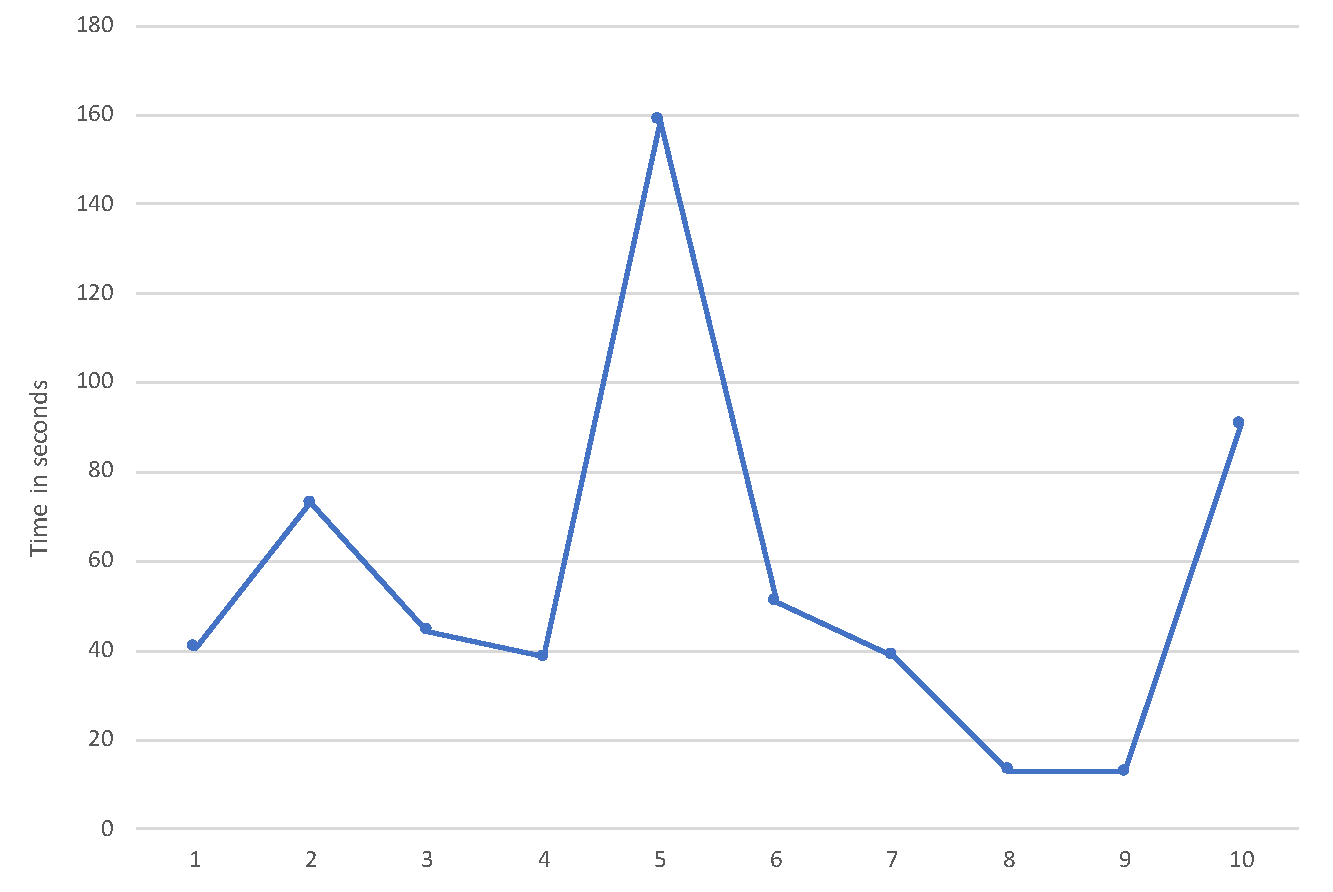
\includegraphics[height=6cm]{./Images/pb-statement-curve.pdf}
	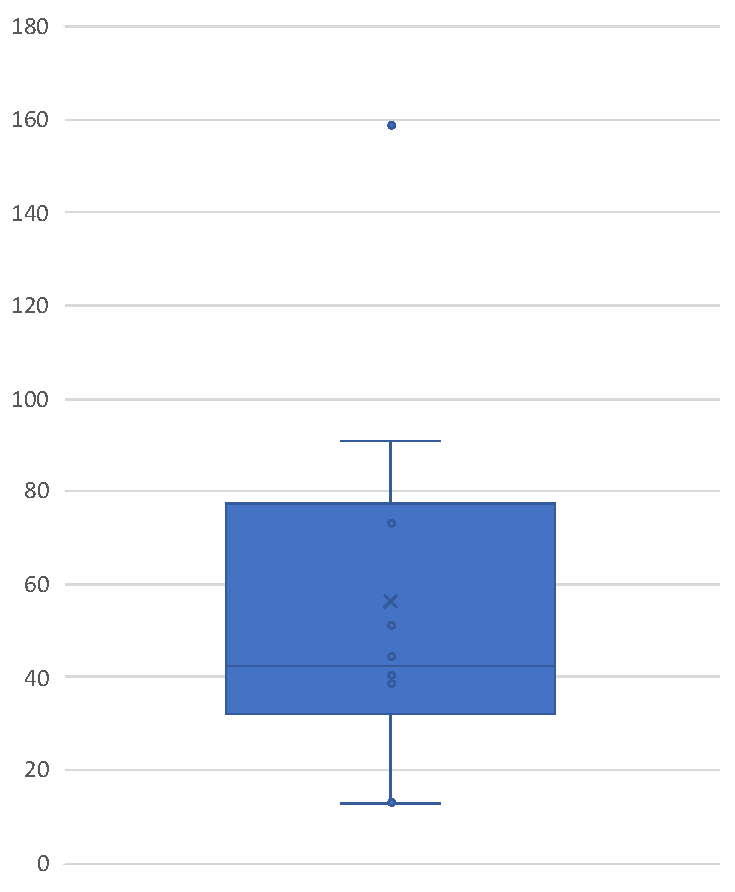
\includegraphics[height=6cm]{./Images/pb-statement-box.pdf}
    \caption{Multiple runs of the same deterministic unit test suite}
    \label{fig:pb-statement}
\end{figure}

The first issue while trying to understand those results is the need of tools
to investigate what is going on under the hood. The second issue is by the
nature of LuaJIT (mostly a one-man job) the documentation is very thin and a bit
scattered all over the place (wiki, website, mailing list, etc.), making life
difficult for newcomers to understand its mechanism.
This is where this project takes place. This part will present analysis of those
instability and provide potential explanations, while the second part
will present my technical understanding of LuaJIT in a structured way to allow
it to be used as a reference for future newcomers, internally at CERN or for any
interested people.
